 % !TEX TS-program = pdflatex
% !TEX encoding = UTF-8 Unicode

% This is a simple template for a LaTeX document using the "article" class.
% See "book", "report", "letter" for other types of document.

\documentclass[a4paper]{article} % use larger type; default would be 10pt

\usepackage[utf8]{inputenc} % set input encoding (not needed with XeLaTeX)

%%% Examples of Article customizations
% These packages are optional, depending whether you want the features they provide.
% See the LaTeX Companion or other references fol\texttt{}r full information.

%%% PAGE DIMENSIONS
\usepackage{geometry} % to change the page dimensions
\geometry{a4paper} % or letterpaper (US) or a5paper or....
% \geometry{margin=2in} % for example, c\texttt{}hange the margins to 2 inches all round
% \geometry{landscape} % set up the page for landscape
%   read geometry.pdf for detailed page layout information

\usepackage{graphicx} % support the \includegraphics command and options

% \usepackage[parfill]{parskip} % Activate to begin paragraphs with an empty line rather than an indent

%%% PACKAGES
\usepackage{booktabs} % for much better looking tables
\usepackage{array} % for better arrays (eg matrices) in maths
\usepackage{paralist} % very flexible & customisable lists (eg. enumerate/itemize, etc.)
\usepackage{verbatim} % adds environment for commenting out blocks of text & for better verbatim
\usepackage{subfig} % make it possible to include more than one captioned figure/table in a single float
% These packages are all incorporated in the memoir class to one degree or another...
\usepackage{caption}
%%% HEADERS & FOOTERS
\usepackage{fancyhdr} % This should be set AFTER setting up the page geometry
\pagestyle{fancy} % options: empty , plain , fancy
\renewcommand{\headrulewidth}{0pt} % customise the layout...
\lhead{}\chead{}\rhead{}
\lfoot{}\cfoot{\thepage}\rfoot{}
\usepackage{pdfpages}
%%% SECTION TITLE APPEARANCE
\usepackage{sectsty}
\usepackage{amsmath}
\usepackage{float}
\usepackage{graphicx}


\usepackage{amssymb}
\usepackage[ngerman]{babel}
\usepackage{float}
\usepackage{svg}
\usepackage{amssymb}

% (This matches ConTeXt defaults)
\setcounter{tocdepth}{4}  % = Aufnahme in das Inhaltsverzeichnis *
\setcounter{secnumdepth}{4} %  = Nummerierung vertiefen *
%%% ToC (table of contents) APPEARANCE
\usepackage[nottoc,notlof,notlot]{tocbibind} % Put the bibliography in the ToC
\usepackage[titles,subfigure]{tocloft} % Alter the style of the Table of Contents
\renewcommand{\cftsecfont}{\rmfamily\mdseries\upshape}
\renewcommand{\cftsecpagefont}{\rmfamily\mdseries\upshape} % No bold!
\usepackage{epstopdf}
%%% END Article customizations
\usepackage{titling}
%%VL UNNOETIG
\usepackage{colortbl}
\usepackage[utf8]{inputenc}
\usepackage[upright]{fourier}
\usepackage{tikz}
\usetikzlibrary{matrix,arrows,decorations.pathmorphing}

\usetikzlibrary{matrix} 

\usepackage[utf8]{inputenc}
\usepackage[upright]{fourier}
\usepackage{tikz}
\usetikzlibrary{matrix}
\usepackage{fullpage,amsmath}


%%% Rand und so
\usepackage{geometry}
\geometry{
	left=3cm,
	right=3cm,
	top=2cm,
	bottom=4cm,
	bindingoffset=5mm
}

\setlength{\parindent}{4em}
\setlength{\parskip}{1em}

\begin{document}

\begin{titlepage}
	\title{Mathematik der Oberstufe}
	\author{Thomas Dost}
	\date{} % Activate to display a given date or no date (if empty),
	\maketitle
	\newpage
	\tableofcontents
	\newpage
\end{titlepage}
	\section{Analysis}
	\subsection{Lineare Funktionen}
	\begin{tabular}[t]{lr}
	Eine lineare Funktionen ist eine Funktion der Form $ f(x)= mx+b$.
	\end{tabular}
	\subsubsection{Eigenschaften einer linearen Funktionen}
	Bei einer Linearen Funktion stellt $m$ die Steigung und $b$ die Verschiebung auf der Y-Achsen dar.
	Die \textbf{Steigung} $m$ einer linearen Funktion $ f(x)= mx+b$ berechnet sich durch $m =\frac{\Delta y}{\Delta x}  = \frac{ y_{2}-y_{1} }{x_{2}-x_{1} }$
	
	\begin{tabular}[t]{lr} 
	\end{tabular}
	
	\begin{minipage}{0.5\textwidth}
		\begin{figure}[H]
			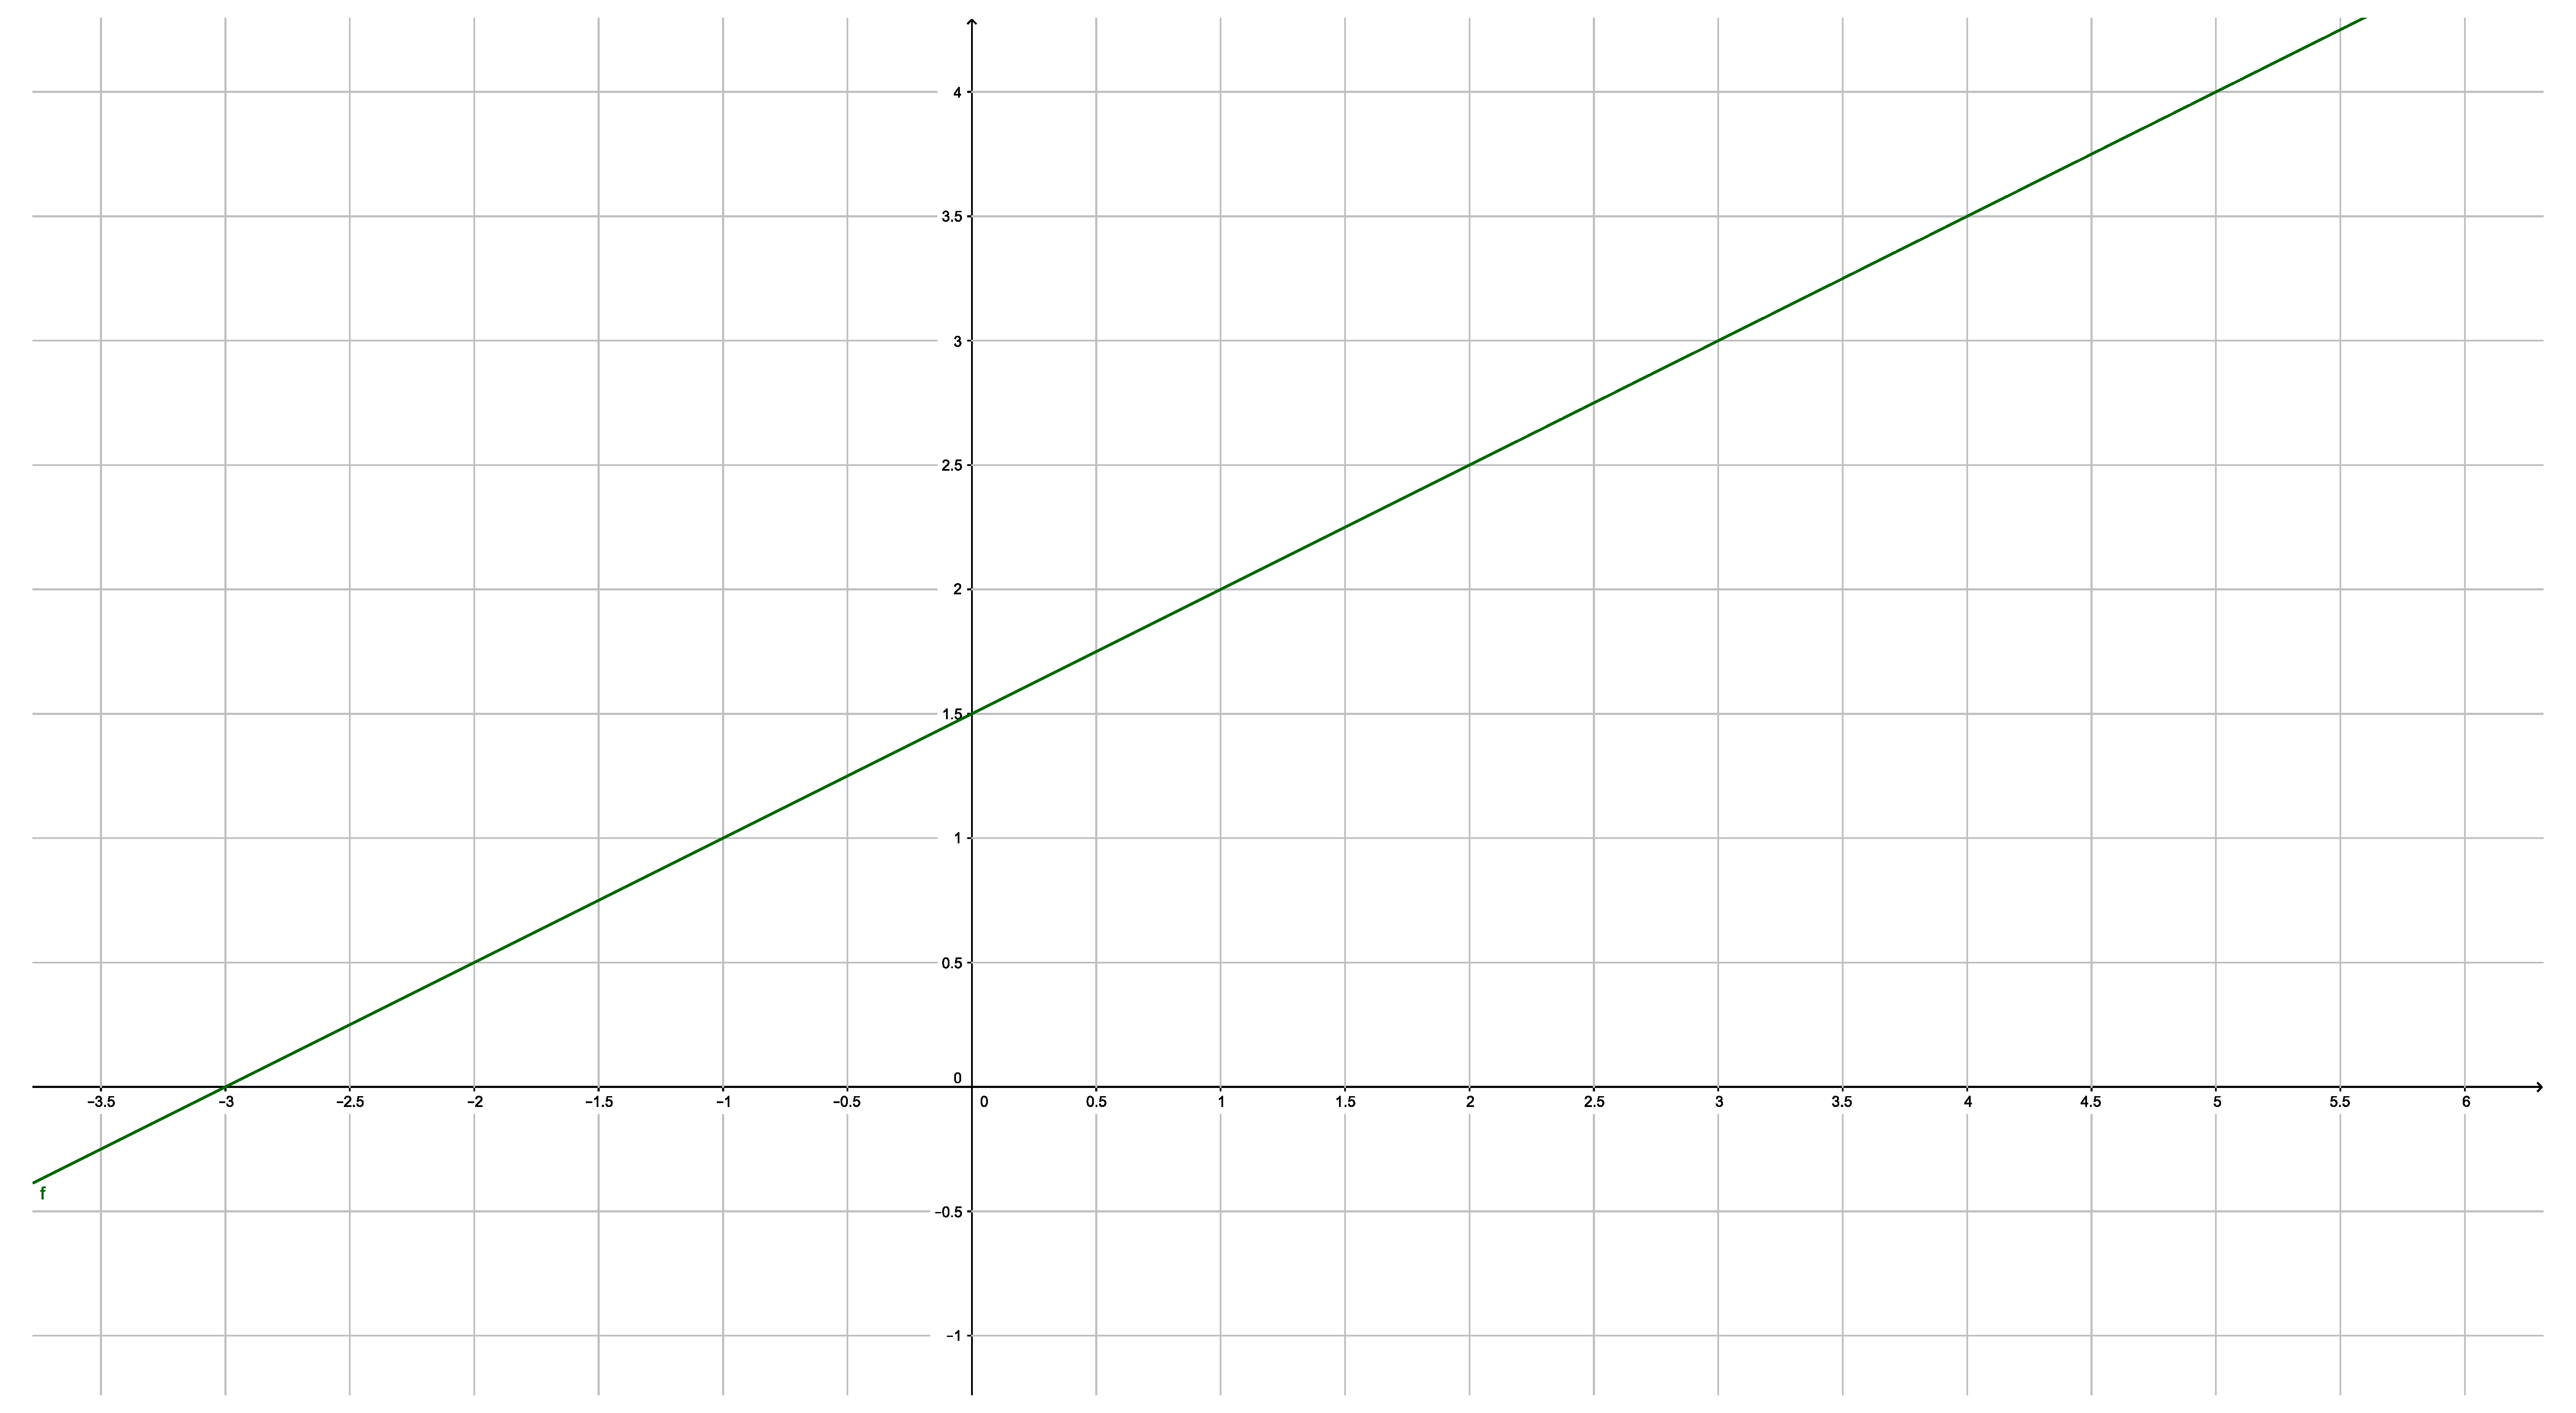
\includegraphics[width=200px, height=200px]{lineare.pdf}
			\captionsetup{labelformat=empty}
			\caption{\label{fig:blue_rectangle} $f(x)=0,5x+1,5$}
		\end{figure}
	\end{minipage} \hfill
	\begin{minipage}{0.45\textwidth}

	Beispiel: 
		\begin{alignat*}{4} 
		m &=\frac{\Delta y}{\Delta x} = \frac{ y_{2}-y_{1} }{x_{2}-x_{1} } \\
		  &\leftrightarrows \frac{3,5 - 1,5}{4 - 0} = 0,5
		\end{alignat*} 
	\end{minipage}
	\newpage
	\subsubsection{Schnittpunkt zweier linearer Funktionen}
		\begin{tabular}[t]{llr} 
			Der \textbf{Schnittpunkt} $x$ zweier linearer Funktonen berechnet sich durch das Gleichsetzen\\ zweier lineare Funktionen:\\
			$f(x) = 0,5x+1,5$\\
			$g(x) = 1x+0,2$
	
		\end{tabular}
		
		\begin{minipage}{0.5\textwidth}
			\begin{figure}[H]
				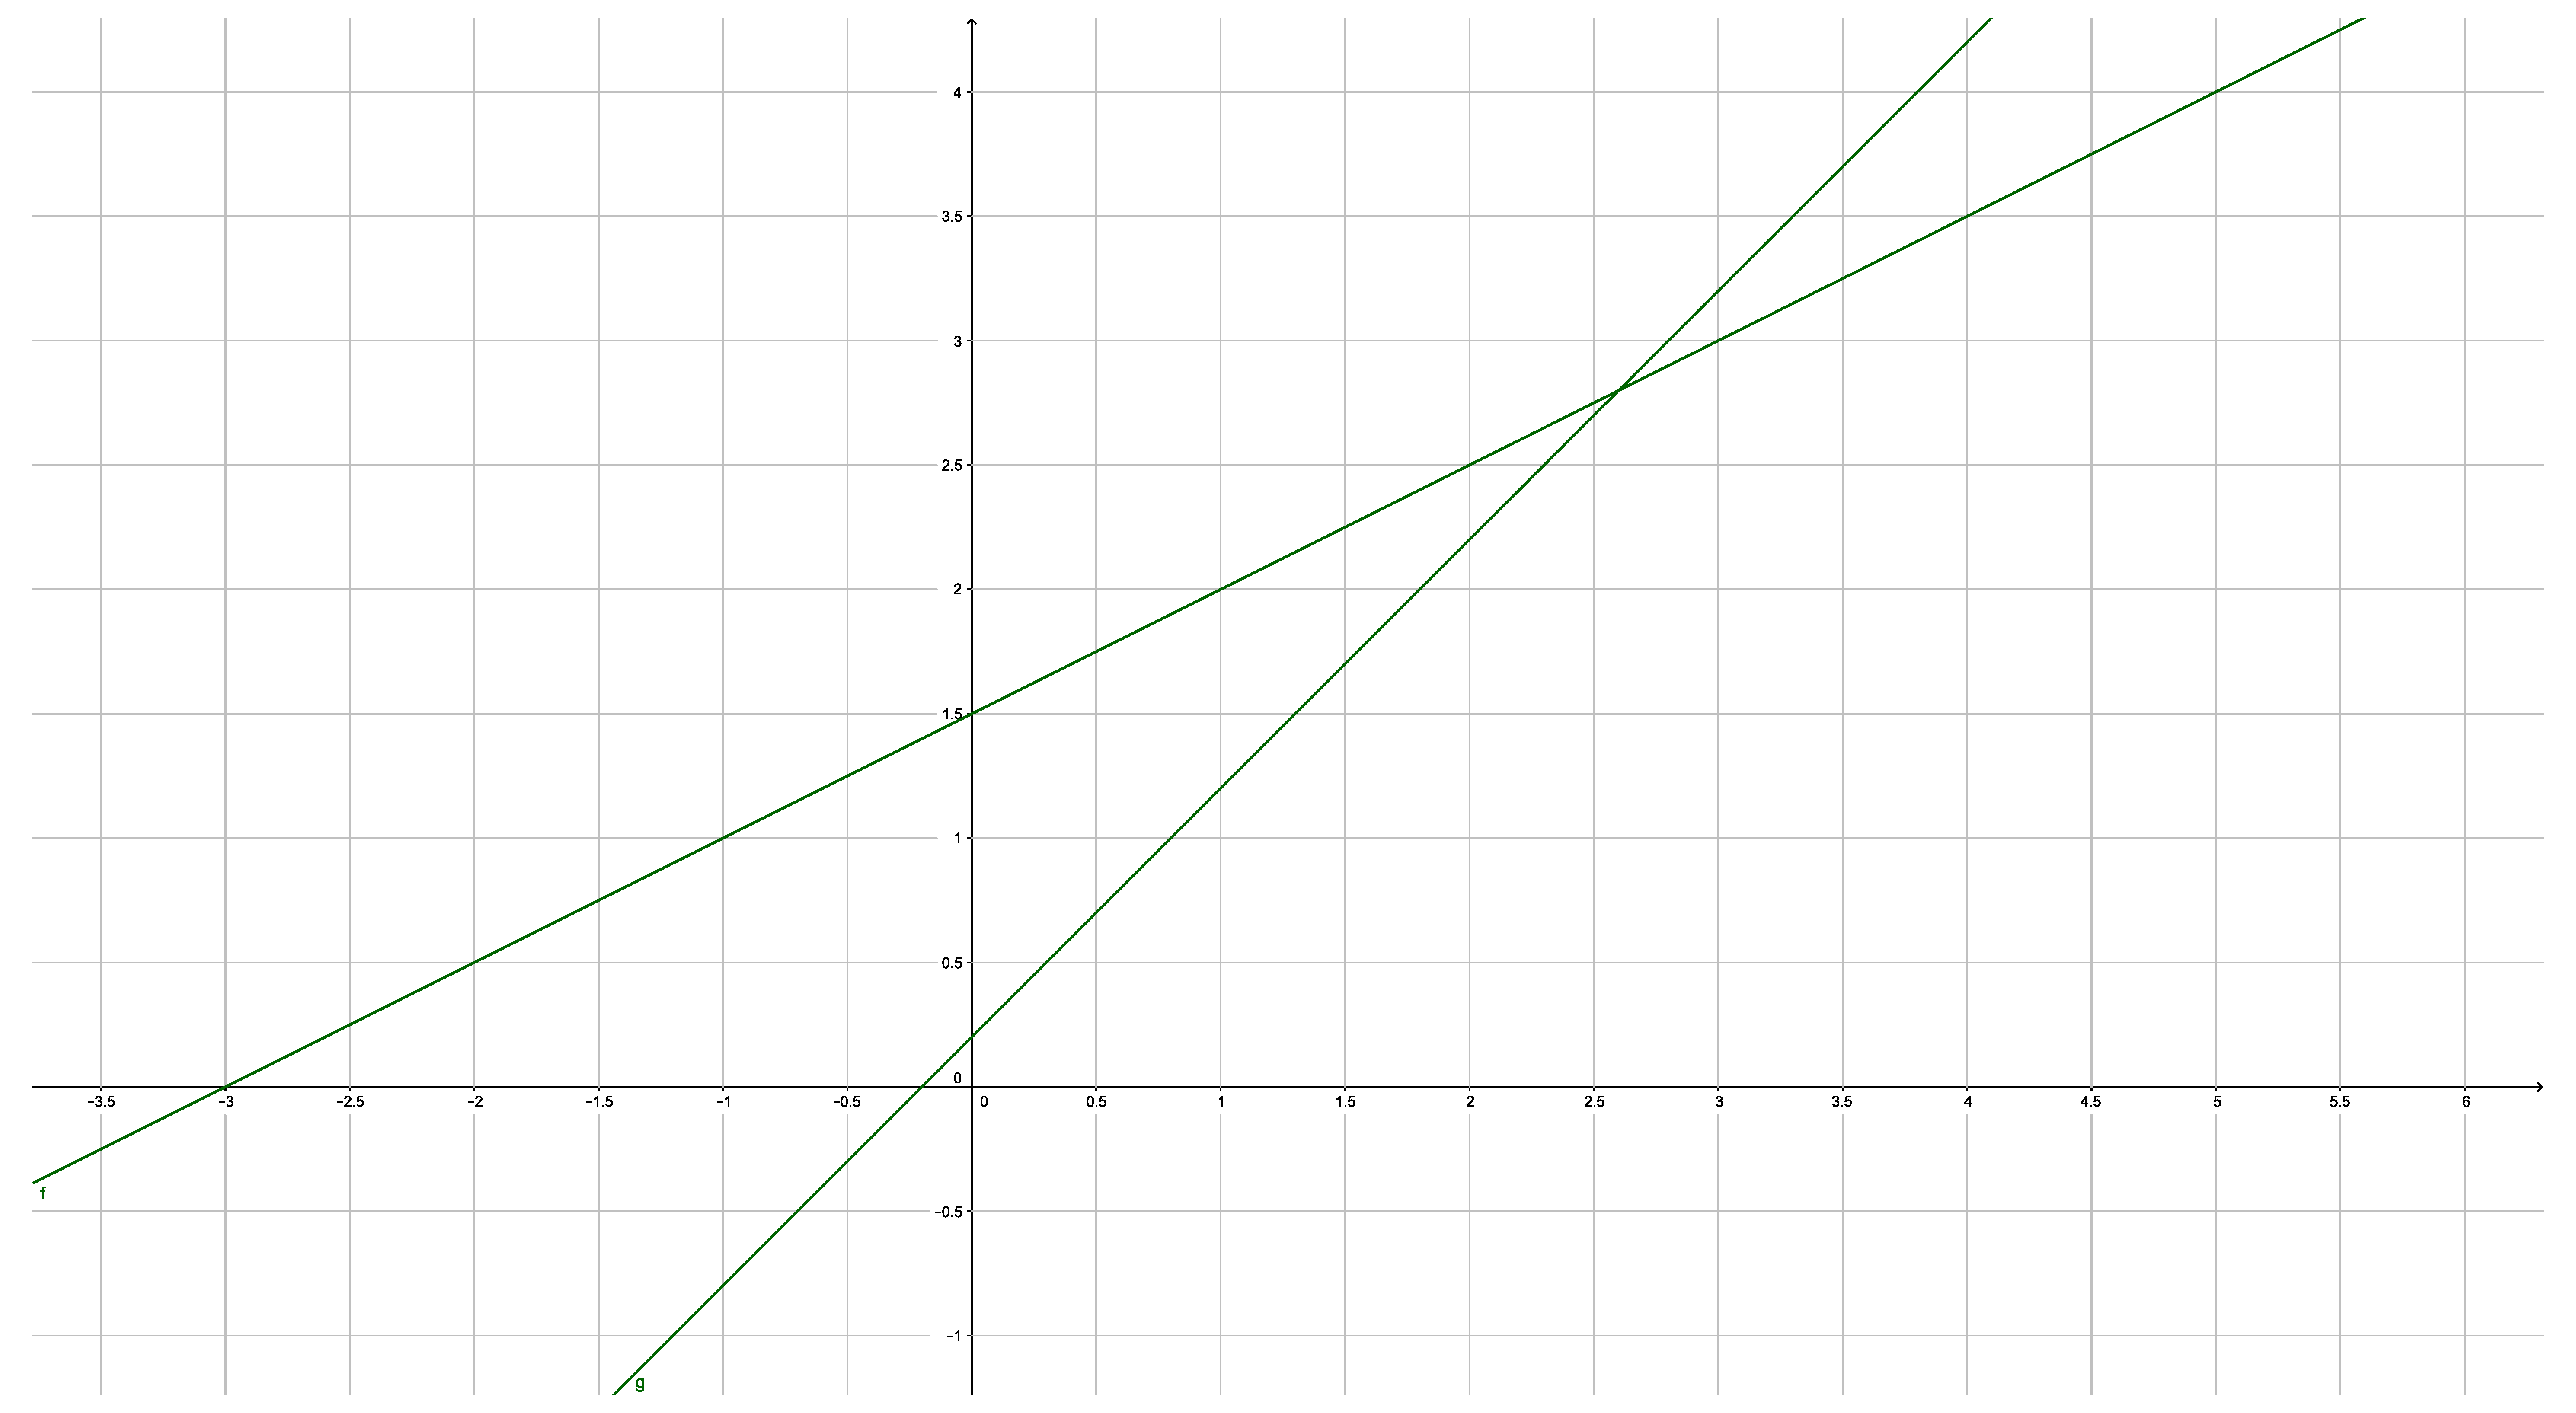
\includegraphics[width=200px, height=200px]{lineare2.pdf}
					\captionsetup{labelformat=empty}
				\caption{  }
			
			\end{figure}
		\end{minipage} \hfill
		\begin{minipage}{0.45\textwidth}
				Beispiel:
			\begin{alignat*}{4} 
			0,5x+1,5 &= 1 && x +0,2 && |-0,5x \\ 
			1,5 	 &= 0,5 && x+0,2 && |-0,2\\ 
			1,3 	 &= 0,5 && x &&|*2 \\
			2,6		 &=  && x  
			\end{alignat*} 
				Jetzt kann das Ergebnis\\($x=2,6$) in die Gleichungen eingesetzt werden um das Ergebnis zu ueberpruefen.\\
				$f(2,6) = 2,8$\\
				$g(2,6) = 2,8$\\
				Da die beiden Werte gleich sind heisst das, dass die Rechnung korrekt ist.
		
		
		\end{minipage}
	\newpage
	\subsection{Quadratische Funktionen}
	\begin{tabular}[t]{llr} 
			Eine quadratische Funktionen ist eine Funktion der Form $ f(x)= ax^{2}+bx+c$ in der Normal\\ -und $f(x) = a(x-x_s)^{2}+y_s$ in der Scheitelpunktform.
		\end{tabular}\\
		\begin{tabular}[t]{llr} 
		\begin{minipage}{0.5\textwidth}
			\begin{figure}[H]
				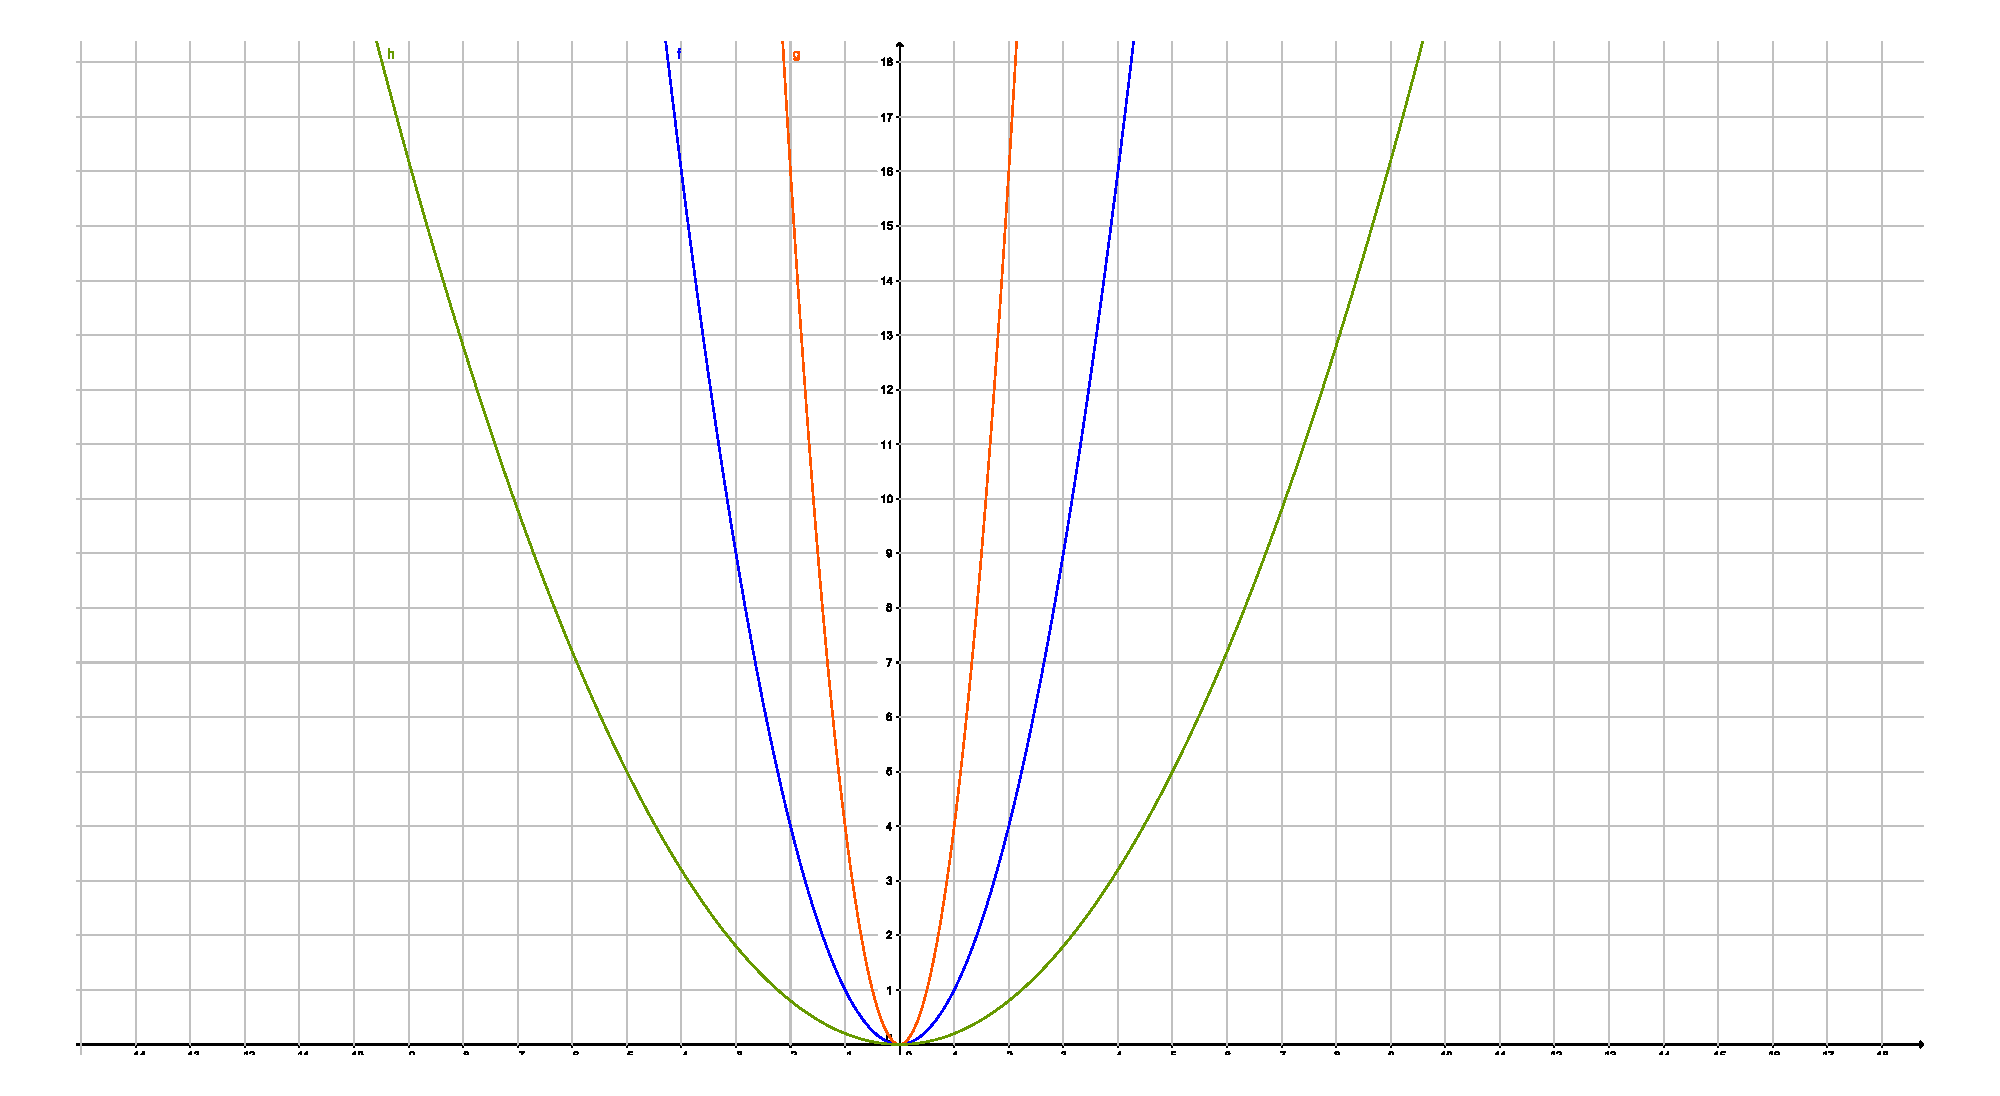
\includegraphics[width=200px, height=200px]{quadr-B.pdf}
				
				\captionsetup{labelformat=empty}
				\centering
				\caption{Gestreckte Parabel:\\  $h(x) =0,2x^{2}+0x+0; \hspace{0,3 cm} 0,2(x-0)^2+0$ } 
				\vspace{-0,3 cm}
				\caption{Normale Parabel:\\ $f(x) =1x^2+0x+0; \hspace{0,3 cm}1(x-0)^2+0  $}
				\vspace{-0,3 cm}
				\caption{Gespreizte Parabel\\ $g(x)=4x^2+0x+0; \hspace{0,3 cm}4(x-0)^2+0 $}
			
			\end{figure}
		\end{minipage} 
		\end{tabular}
		\begin{minipage}[t]{0.5\textwidth}
			\vspace{-3.8 cm}
			
		\end{minipage}	
	
	\subsubsection{Eigenschaften einer quadratischen Funktionen}
	Die Verschiedenen Koeffinzienten einer quadratichen Funktion, haben verchiedene Auswirkungen auf das Aussehen einer
	quadratischen Funktion.\\
	\\ \textbf{Normalform:}\\
	Der \textbf{Koeffizient $a$} gibt sowohl die Oeffnungsrichtung als auch die Steigung einer Parabel wieder, ist $a < 0$ ist die Parabel nach unten geoeffnet, ist $a > 0$ ist sie nach oben geoeffnet. Ist $a = 0$ ensteht eine lineare Funktion.\texttt{}\\
	Ueber die Steigung kann man folgene Aussagen treffen: Ist $a > 1$ ist die Parabel gestreckt, ist $a<1$ ist sie gespreitzt, $a=1$ stellt die Normalparabel da.
	\\\\Der \textbf{Koeffinzienten $b$} gibt die Steigung der Parabel im Schnittpunkt mit der y-Achse an, zusaetlich laesst sich am Vorzeichen ablesen
	ob die Parabel die Y-Achse(Ordinatenachse), mit dem fallenden Ast der Parbel geschnitten wird oder mit dem Steigenden.
	Ist $b < 0$, scheidet der fallende Ast die Ordinatenachse, sonst der Andere.
	Eine Veraenderung des Koeffinzienten $b$ bewirkt eine Verschiebung sowohl in x- als auch in y-Richtung. Wird $b$ um eins eroeht, dann wird der Graph um 1/2a Einheiten nach links und (2b+1)/4a nach unten verschoben. Wird b um eins verringert, wird der Graph dagegen um 1/2a Einheiten nach rechts und (2b-1)/4a nach oben verschoben.
	
	

	\hspace{-1.5 cm}
	Der \textbf{Koeffizient $c$} bestimmt wie die Funktion auf der Ordinatenachse verschoben ist.


	\subsubsection{Umwandlung der Normalform in die Scheitelpunktform}
	
		Es sei $f(x)=2x^2+2x+5$, um diese Funktion in die Scheitelpunktform zu ueberfuehren\\ muessen folgende Schritte vollzogen werden.
		
		\begin{alignat*}{4} 
		%%%%%%%%%%%%%%%%%%%%%%%%%%%%%%%%%%%%%%%%%%%%%%%%%%%%
		%Nochmal allgemeingueltig |SP \hspace{0.1 cm} der Funktion, Werte einzs\\
		%%%%%%%%%%%%%%%%%%%%%%%%%%%%%%%%%%%%%%%%%%%%%%%%%%%%5%%
		 f(x) 						&=  (ax^{2}    	     + && bx) 										 	   							  &&+c     && \hspace{0.3 cm}|a \hspace{0.1 cm} ausklammern \\ 
									&= a\bigg( x^{2} 	     + && \frac{b}{a}x \bigg) 						 		   	   							  && +c    && \hspace{0.3 cm}|q.E. \\
									&=  a \bigg[ x^{2}   + && 2\frac{b}{2a}x + \bigg(\frac{b}{2a}\bigg)^2 - \bigg(\frac{b}{2a}\bigg)^2 \bigg]&& +c    && \hspace{0.3 cm}|bin. Form\hspace{0.12 cm} rueckwaerts\\
									&=  a \bigg[\bigg( x + && \frac{b}{2a} \bigg)^{2}  - \bigg(\frac{b}{2a}\bigg)^2 \bigg]				  && +c    && \hspace{0.3 cm}|Klammer\hspace{0.1 cm} aufloesen\\
									&=  a \bigg( x       + && \frac{b}{2a} \bigg)^{2}  - \frac{ab^{2}}{4a^{2}} 							  && +c    && \hspace{0.3 cm}|a \hspace{0.1 cm} kuerzen \\ %%WIE GEHT DAS
									&=  a \bigg( x       + && \frac{b}{2a} \bigg)^{2}  +\bigg( c - \frac{b^{2}}{4a}\bigg) 				  &&       && \hspace{0.3 cm} |SPF \hspace{0.1 cm} der Funktion \\
		\end{alignat*}
		\hspace{-0.1 cm}
		Hier kann man nun den Scheitelpunkt ablesen: \\
		
		S =   $\bigg( -\frac{b}{2a}  | c - \frac{b^{2}}{4a}\bigg)$ =  $\bigg( -0,5  | 4,5\bigg)$ 
		\subsubsection{Schnittpunkt zweier quadratischer Funktionen}
		$f(x)=5x^2-10x+2$\\
		$g(x)=x^2+2x+0$
		
		\begin{align*}
			5x^2-10x+2 &= x^2+2x+0 & 	|&-2x\\
			5x^2-12x+2 &= x^2 & 		|&-x^2\\
			4x^2-12x+2 &= 0   & 		|&:4\\
			x^2-3x+0.5 &= 0 	
		\end{align*}
			Nun kann die Gleichung mit der P-Q-Formel geloest werden.
		\newpage
		\subsection{Funtionen mit dem Grad groesser 2}
		\subsubsection{Substitution}
		\subsubsection{Polynomdivision}
		\subsection{Trigonometrische Funktionen}
		\subsection{Tangente und Normale}
		\subsection{Exponentialfunktionen}
		\subsubsection{Natuerliche Expoentialfunktion}
		Als natuerliche Exponentialfunktion bezeichnet man Variationen der Funtion $f(x)=e^x$.
		\subsection{Umkehrfunktion}
		\subsection{Funktionenscharen}
		\subsection{Herleitung}
		\subsubsection{Trigonometrische Funktionen}
		\subsubsection{Quadratische Ergaenzung}
		\subsubsection{P-Q-Formel}
		\subsubsection{Polynomdivision}
		\subsubsection{Horner Schema}
	\newpage
	\section{Differentialrechnung}
	\subsection{Ableitung}
	\subsection{Visualisierung}
	

	\begin{minipage}{0.3\textwidth}
	\begin{figure}[H]
	\includegraphics[width=300px, height=200px]{a.eps}
	\caption{Rectangle}
	\end{figure}
	\end{minipage} \hfill
	\begin{minipage}{0.5\textwidth}
	
	Hier zu sehen ist der Graph $f(x)$, mit seinen Ableitungen $f'(x)$ und $f''(x)$.
	Hier kann man sehr gut erkennen wie die Nullstellen der 1. Ableitung $f'(x)$, genau an
	der Position liegen an der auch die Steigung von $f(x)$ gleich 0 ist.\\
	Schaut man sich nun die 2. Ableitung an, kann man erkennen das sich Nullstelle der 2. Ableitung an der Stelle befinden wo $f(x)$ eineWendepunkt hat.
	
	\end{minipage}


			
		
%	\end{tabular}
	\subsection{Bedeutung der 1. Ableitung}
	\begin{tabular}[t]{l}
	Die 1. Ableitung gibt die Steigung der Originalfunktion wieder, d.h wenn die 1. Ableitung 0 ist \\hat die Originalfunktion an diesem Punkt eine 
	Steigung von 0 und damit einen moeglichen \\Extrempunkt.
	\end{tabular}
	\subsection{Bedeutung der 2. Ableitung}
	Muss Ueberarbeitete werden\\
	Die 2. Ableitung gibt die Steigung der 1. Ableitung wieder, d.h wenn die 2. Ableitung 0 ist \\hat die 1. Ableitung an diesem Punkt eine 
	Steigung von 0. und damit hat die Originalfunktion an diesem Punkt einen Steigunswechsel
	\subsection{Kurzform des Ableitens}
	
	Das Ableiten besitzt eine Kurzform, ohne jedes mal den Limes benutzen zu muessen, dabei muss man die Ableitungsregeln sowie die Tatsache dass ein konstanten Summand beim Ableiten wegfaellt beachten(Summenregel).
\\	Beispiel:\\
	$f(x)  =5x^2+3x^1-5x^0$\\
	$f'(x)  =2*5x^{2-1}+1*3x^{1-1} = 10x^1+3x^0$\\
	In Worte gefasst bedeutet dass, das der Originalexponent vor den Koeffizenten gezogen und mit diesem multipliziert wird, danach wird der Exponent um 1 dekrementiert.
	\subsection{Ableitungsregeln}
	\subsubsection{Summenregel}
	Summen von Funktionen werden getrennt abgeleitet. \\
	Beispiel: \\ 
		\begin{align*}
			f(x) &= 5x^2+8x  \\
			 f'(x)&= 10x+8
		\end{align*}
	\subsubsection{Faktorregel}
	Konstante Faktoren bleiben beim Ableiten erhalten. \\
	Beispiel: \\ \begin{align*}
					f(x)&= 5*x^2 \\ 
					f'(x) &= 5*2x
				\end{align*}
	
	\subsubsection{Produktregel}
	\begin{align*}
		f(x)&=u(x)*v(x)\\
		f'(x)&=u'(x)*v(x)+u(x)*v'(x)
	\end{align*}
	Beispiel: \\ 
	\begin{align*}
		f(x) &= 5x^2*8x-1  \\
		f'(x)&= 10x*8x+5x^2*8
	\end{align*}
	\subsubsection{Kettenregel}
	"Auesere mal innere Ableitung".\\
	Ist eine Funktion das Ergebnis der Vekettungs von 2 anderen Funktionen dann gilt:\\
	 \begin{align*}
		f(x)&=(u \circ v)(x)\\
		f'(x)&=u'(v(x))*v'(x)
	\end{align*}
	\\Beispiel:\\
		\begin{align*}
		f(x) &=e^{5x}\\
		f'(x)&=5e^{5x}
		\end{align*}

		\begin{align*}
		f(x)&=sin(5x)\\
		f'(x)&=5*cos(5x)
		\end{align*}

	\subsubsection{Quotientenregel}
		\begin{align*}
		f(x)&=\frac{u(x)}{v(x)}\\
		f'(x)&=\frac{u'(x)*v(x)-u(x)*v'(x)}{(v(x))^2}
		\end{align*}
		Beispiel: \\ 
	
	\subsection{Ableitung der $e$-Funktion}
	Die Ableitung der Funktion $f(x)=e^x$ ist $f'(x)=e^x$
	\\Beispiel:\\
	\begin{align*}
		f(x)&=5e^x\\
		f'(x)&=5e^x
	\end{align*}
	\subsection{Ableitung trigonometrischer Funktionen}
	\subsection{Herleitungen}
	\subsubsection{Herleitung der Ableitung mithilfe des Limes}
	\subsubsection{Herleitung der Potenzregeln in  $\mathbb{N}$}
	\subsubsection{Herleitung der $e$-Funktion in der Menge der natuerliche Exponenten}
	\subsubsection{Herleitung der Trigofunktion mithilfe des Limes}
	\subsubsection{Herleitung der Ableitungsregeln}
	\section{Integralrechnung}
	TEST

	\subsection{Rotationskoerper}  
	HALLO GITHUB                                                       
	\subsection{Herleitungen}
	\section{Kurvendiskussion}
	\subsection{Symmetrie}
	\subsection{Verhalten im Unendlichen}
	\subsection{Schnittpunkt mit der y-Achse}
	\subsection{Nullstellen}
	\subsection{Ableitungen}
	\subsection{Extrema berechnen}
	\subsection{Wendepunkte berechnen}
	\section{Analytische Geometrie}
	\subsection{Was ist ein Vektor}
	Ein Vektor ist eine Menge von Pfeilen der Form $\vec{a} = \begin{pmatrix} a_1 \\ \vdots \\ a_n \end{pmatrix} $, die parallel untereinander verschoben sind.
	Eine anderen Notation fuer diesen Vektor waere $\vec{a} = \begin{pmatrix} a_1  \hdots  a_n \end{pmatrix}^T $
	\subsection{Koordinatensystem}
	\begin{minipage}{0.5\textwidth}
			\begin{figure}[H]
				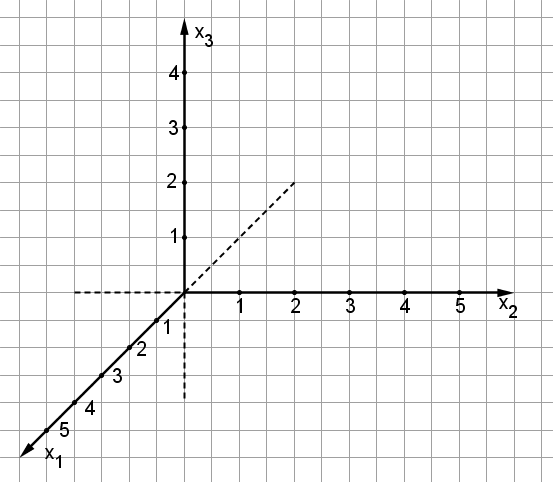
\includegraphics[width=200px, height=200px]{koordinatensystem.png}
					\captionsetup{labelformat=empty}
				\caption{3D Koordinatensystem}
			\end{figure}
		\end{minipage} 
	\subsection{Besondere Vektoren}
	\subsubsection{Nullvektor}
	Der Nullvektor ist ein Vektor der Form $\vec{v} = \begin{pmatrix} 0 \\ \vdots \\ 0 \end{pmatrix}$, 
	 zudem ist er das neutrale Element der Vektoraddition d.h. $ \vec{a} + \begin{pmatrix} 0 \\ \vdots \\ 0 \end{pmatrix} = \vec{a}$.
	\subsubsection{Gegenvektor}
	Der Gegenvektor ist das inverse Element der Vektoraddtion d.h $ \vec{a}+ -\vec{a}=0$, wobei - $0$ den Nullvektor bezeichnet.
	\subsubsection{Ortsvektor}
	Ein Ortsvektor beziehcnet einen Vektor der vom Koordinatenursprung aus geht d.h. er hat die Form $\vec{OP}$, wobei $P$ ein beliebiger Punkt im Raum ist.
	\subsubsection{Normalenvektor}
	Ein Normalenvektor ist ein Vektor der orthogonal zu seinem Bezugsobjekt z.B. einer Gerade ist. 
	\subsubsection{Einheitsvektor}
	Ein Einheitsvektor ist ein Vektor der Laenge 1, d.h. dass sein Betra5z5g = 1 ist($|\vec{a}|=1$).
	\subsection{Rechnen mit Vektoren}
	\subsubsection{Addition}
	Zwei Vekotren in $\mathbb{R}^3$ $\vec{a}, \vec{b}$ werden addiert, idem man ihre Komponenten addiert.
	\\Beipsiel
	$\vec{a}+\vec{b}=\begin{pmatrix}a_1\\a_2\\a_3\end{pmatrix}+\begin{pmatrix}b_1\\b_2\\b_3\end{pmatrix}=\begin{pmatrix}a_1+b_1\\a_2+b_2\\a_3+b_3\end{pmatrix}$
	\subsubsection{s-Multilipkation}
	Ein Vektor $\vec{a}$ wird mit einer Zahl $s$ aus $\mathbb{R}$ multipliziert, in dem seine Komponenten mit $s$ multipliziert werden.
	$s*\vec{a}=s*\begin{pmatrix}a_1\\a_2\\a_3\end{pmatrix}=\begin{pmatrix}s*a_1\\s*a_2\\s*a_3\end{pmatrix}$
	\subsubsection{Linearkombination}
	Einen Ausdruck der Form $r_1*\vec{a}_1 + r_2*\vec{a}_2 + \hdots + r_n*\vec{a}_n $ nennt man Linearekombination der Vektoren $a_1$ bis $a_n$.
	Beachte das $a_1$ bis $a_n$ Vektoren, und keine Vektorkomponenten sind.
	\subsubsection{Laenge eines Vektors}
	Der Betra eines Vektors $\vec{a}$ stellt seine Laege da, d.h. $|a|=\sqrt{a_1^2+a_2^2+a_3^2}$ ist die Laenge eines Vektors.
	\subsubsection{Skalarprodukt}
	Das Sklalarprodukt ordnet je zwei Vektoren $\vec{a},\vec{b}$ ein Sklalar zu, ist dieses Skalar $0$ sind die Vektoren orthogonal zueinander, ist es $< 0$ sind sie parallel und gleichorientiert, ist es $> 0$, sind sie parallel und entgegengesetzt orintiert. Es wird folgendermaßen berechntet: $\vec{a} \circ \vec{b}=a_1*b_1+a_2*b_2+a_3*b_3$.
	\subsubsection{Kreuzprodukt}
	\paragraph{Berechnung mithilfe Determinante}
	\subsubsection{Spatprodukt}
	\subsection{Geraden}
	\subsubsection{Was sind Geraden}
	\subsubsection{Lage von zwei Geraden im Raum}
	\paragraph{Parallel}
	\paragraph{Identisch}	
	\paragraph{Windschief}
	\paragraph{Schnittpunkt}
	\paragraph{Winkel zwischen Gerade}
	\subsection{Ebenen}
	Eine Ebene im 3-Dimensionalen Raum ist eine uendliche Ausdehnung in zwei Richtungen.
	\begin{figure}[H]
				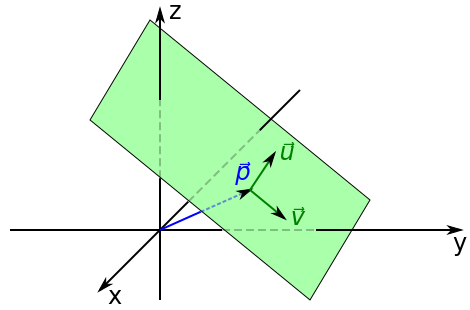
\includegraphics[width=150px, height=150px]{Ebene.png}$^{[5]}$
					\captionsetup{labelformat=empty}
				\caption{Ebene im 3-Dimensionalen Raum}
	\end{figure}
	\subsubsection{Ebenenformen}
	\paragraph{Parameterform}
		\hspace{0 cm} \\ \noindent \\
	Paramterform einer Ebene: $E : \vec{x} = \vec{p}+ r*\vec{u}+s*\vec{v}$\\
	In der Paramterform wird eine Ebene mithilfe eines Stuetzvektors(Ortsvektors) und zwei Richtungsvektoren beschrieben.
	Es gibt zwei Moeglichkeiten wie diese Richtungsvektoren zueiander liegen duerfen um eine Ebene zu beschreiben.
	\\\\Geschitten\\
	Falls sich die gegebenen Richtugnsvektoren schneiden, kann die Ebene direkt zwischen ihnen aufgespannt werden.
	\\Beispiel
	\\\textbf{\\Parallel}\\
	Falls die gegeben Richtungsvektoren jedoch Parallel sind, muss ein Verbindungsvektor zwischen ihen hergestellt werden.
	\\Beispiel
	\paragraph{Normalenform}
	\paragraph{Koordinatenform}
	\paragraph{Hess'che Normalenform}
	\subsubsection{Lage Ebene Gerade}
	\paragraph{Parallel}
	\paragraph{Schnittpunkt}
	\paragraph{Winkel zwischen Gerade und Ebene}
	\subsubsection{Lage Ebene Ebene}
	\paragraph{Parallel}
	%\subparagraph{Identisch}
	\paragraph{Schnittpunkt}
	\paragraph{Winkel zwischen Ebenen}
	\subsubsection{Abstandsberechnung im Raum}
	\subsection{Kugeln}
	\subsubsection{Was ist eine Kugel}
	Eine Kugel ist eine Menge von Punkten im 3-Dimensionalen Raum, die von einem festen Punkt $M$ den gleichen Abstand $r$ haben,
	der Punkt $M$ wird dabei als Mittelpunkt und der Abstand $r$ als Radius bezeichnet.
	\subsubsection{Kugelgleichung}
	Eine Kugel in der Analytischen Geometrie wird mit der Gleichung\\ $|\vec{p}-\vec{M}|^2=r^2$ oder
	$(p_1-M_1)^2+(p_2-M_2)^2+(p_3-M_3)^2=r^2$ beschrieben, wo $M$ den Mittelpunkt als Vektor, $p$ einen beliebigen Punkt als Vektor, und $r$ den Radius als reele Zahl darstellt.
	\subsubsection{Lage Kugel Punkt}
	\subsubsection{Lage Kugel Gerade}
	\paragraph{Schnittpunkt}
	\subsubsection{Lage Kugel Ebene}
	\paragraph{Schnittebene}
	\subsubsection{Lage Kugel Kugel}
	\paragraph{Schnittvolumen}
	\subsection{Herleitungen}
	\subsubsection{Satz des Pythagoras}
	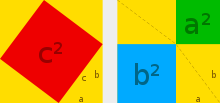
\includegraphics[width=220 px, height=103 px]{pytha.png}\\
	Links = $c^2+ 4*(\frac{1}{2}a*b)$\\
	Rechts = $a^2-b^2+4*(\frac{1}{2}a*b)$

	\begin{align*}
	c^2+ 4*(\frac{1}{2}a*b) &= a^2+b^2+4*(\frac{1}{2}a*b)  \hspace{0.5 cm} |-4*(\frac{1}{2}a*b)\\
	c^2 &= a^2+b^2
	\end{align*}


	
	
	\subsubsection{Pythagoras im Raum}
	\subsubsection{Kosinussatz}
	\subsubsection{Skalarprodukt}
	\subsubsection{Kreutzprodukt}
	\subsubsection{Spatprodukt}
	\subsubsection{Hess'sche Normalform}
	\section{Lineare Algebra}
	\subsection{Loesungsverfahren fuer LGS}
	\subsubsection{Treppenstuffen Verfahren}
	\subsubsection{Koeffizienten Matrix}
	\subsubsection{Determinante}
	\pagebreak
	\subsection{Matrizen}
	 \hspace{0 cm} 
	Eine Matrix vom Typ $M_{m,n}$ ist eine Zusammenfassung von Werten der Form $M =$
	$
	\begin{pmatrix}
		a_{11} & a_{12} & ... 	& a_{1n}\\
		a_{21} & a_{22} & ...		 & a_{2n}\\
	      \vdots    	&      &	    \\
		a_{m1} & a_{m2} & ...	& a_{mn}
	\end{pmatrix}
	$\\
	 mit $m$ Zeilen und $n$ Spalten
	\subsubsection{Besondere Matrizen}
		\paragraph{Nullmatrix  } 
		\hspace{0 cm} \\ \noindent \\
		Die Nullmatrix ist eine Matrix in der alle Elemente Null sind, sie ist damit das neutrale Element der Matrixaddition.\\
		\\$M =$
		$
		\begin{pmatrix}
		0 & 0 	& ... 	& 0\\
		0 & 0 	& ...	& 0\\
		\vdots  &      	&  \\
		0 & 0	& ...	& 0
		\end{pmatrix}
		$\\
	
	\paragraph{Stochastische Matrix  } 
	\hspace{0 cm} \\ \noindent \\
	Eine Stochastische Matrix ist eine quadratische Matrix deren Elemente zweischen 0 und 1 liegen, und der Spalten bzw. Zeilensumme 1 ist.
	
	\paragraph{Inverse  } 
	 \hspace{0 cm} \\ \noindent \\
	 Seien  $M$ und $I$ beliebige quadratische Matrizen und $E$ die Einheitsmatrix, dann nennt man die Matrix $I$ die, die Gleichung $M*I=I*M=E$ erfuellt, Inverse der Matrix $M$. Sie wird mit $M^{-1}$ dargestellt.\\\\
	 Beispiel:\\
	 Eine Matrix mit einer Inversen nennt man regluaere Matrix.
	
	\paragraph{Einheitsmatrix} 
	 \hspace{0 cm} \\ \noindent \\ Eine Einheitsmatrix ist eine quadratische Matrix, bei der alle Elemente auf der Hauptdiagonale gleich 1 sind.\\
	Sie ist das neutrale Element der Matrizenmultiplikation d.h. $M*E = E*M = M$ wobei $M$ eine beliebige regulaere Matrix ist, und $E$ ihre Einheitsmatrix ist.\\
	Sie ist symmetrisch, d.h $E^{t}=E$.\\
	Sie ist selbstinvers, d.h $E^{-1}=E$\\
	Ihre determinante ist 1 d.h $det(E)=1$\\\\
	$E =$
		$
		\begin{pmatrix}
		1 & 0 	& ... 	& 0\\
		0 & 1 	& ...	& 0\\
		\vdots  &     	& \ddots  \\
		0 & 0	& ...	& 1
		\end{pmatrix}
		$\\

	\newpage
	\paragraph{Fixvektor}
		\hspace{0 cm} \\ \noindent \\
	Sei  $V_f$ ein Vektor, und $M$ eine beliebige Matrix, dann nennt man den Vektor der die Gleichung \\	$M * V_f = V_f$ erfuellt Fixvektor der Matrix M.\\\\
	Beispiel:

	\paragraph{Grenzmatrix}
	 \hspace{0 cm} \\ \noindent \\
	Sei $M$ eine beliebige Matrix, dann nennt man eine Matrix die Gleichung $M * M = M$ erfuellt Grenzmatrix der Matrix $M$.
	\\\\
	Beispiel:
	\newpage
	\subsubsection{Rechenregeln}
	\textbf{Addition}\\
	Die Summe zweier Matrizen, berechnet man in dem man sie komponentenweise addiert.\\\\
	\small
	$M = A + B = $ 	
	$
	\begin{pmatrix}
		a_{11} & a_{12} & ... 	& a_{1n}\\
		a_{21} & a_{22} & ...	& a_{2n}\\
		\vdots &        &	    &\\
		a_{m1} & a_{m2} & ...	& a_{mn}
	\end{pmatrix}
	$
	+
	$
	\begin{pmatrix}
	b_{11} & b_{12} & ... 	& b_{1n}\\
	b_{21} & b_{22} & ...	& b_{2n}\\
	\vdots &        &	    &\\
	b_{m1} & b_{m2} & ...	& b_{mn}
	\end{pmatrix}
	$
	=
	$
	\begin{pmatrix}
	a_{11}+b_{11} & a_{12}+b_{12} & ...    & a_{1n}+b_{1n}\\
	a_{21}+b_{21} & a_{22}+b_{22}  & ...	   & a_{2n}+ b_{2n}\\
	\vdots        &               &	       &\\
	a_{m1}+b_{m1} & a_{m2}+b_{m2} & ...	   & a_{mn}+ b_{mn}
	\end{pmatrix}
	$\\
	\\
	Die Matrixaddition ist sowohl \textbf{kommutativ}$(A+B=B+A)$,\\ als auch \textbf{assoziativ}$( (A+B)+C = A +(B+C))$.\\
	Es koennen nur Matrizen der gleiche Dimension addiert werden.\\\\
	\textbf{Skalarmultiplikation}\\
	
		$r * M = r * $ 	
		$
		\begin{pmatrix}
		a_{11} & a_{12} & ... 	& a_{1n}\\
		a_{21} & a_{22} & ...	& a_{2n}\\
		\vdots &        &	    &\\
		a_{m1} & a_{m2} & ...	& a_{mn}
		\end{pmatrix}
		$
		=
		$
		\begin{pmatrix}
		r*a_{11} & r*a_{12} & ... 	& r*a_{1n}\\
		r*a_{21} & r*a_{22} & ...	& r*a_{2n}\\
		\vdots &        &	    &\\
		r*a_{m1} & r*a_{m2} & ...	& r*a_{mn}
		\end{pmatrix}
		$
		\\\\\\
		\textbf{Matrizenmultiplikation}\\
		Zwei Matrizen werden multipliziert indem man das Skalaprodukt von den Zeilenvektoren der erstem Matrix\\
		Es koennen nur Matrizen multipliziert wenn die \textbf{Spaltenanzahl} der 1. Matrix mit der \textbf{Zeilenanzahl} der 2. Matrix uebereinstimmt.\\
		Die Matrizenmultiplikation ist im allgemeinen\textbf{ nicht} kommutativ$(A*B\neq B*A)$, daraus folgt dass beim \textbf{Distributivgesetz} die Richtung eine Rolle spielt$(A*(B+C)\neq (B+C)*A)$.
	

		\begin{tabular}{c|c}
		$A_{2,3}*B_{3,4} = C_{2,4}$  & 		


		
		$\left(\begin{array}{cccc}
			a_{11} 	&  a_{12}  &	a_{13} 	&	 a_{14}  \\ 
			a_{21}  &  a_{22}  &	a_{23} 	&	 a_{24}  \\
			a_{31}  &  a_{32}  &	a_{33}  &	 a_{34}  \\
		\end{array}\right)$ \\
		\hline \\
		
		
		$				 
		\left(\begin{array}{ccc}
		 b_{11} 	&  b_{12} &	b_{13}\\  
		 b_{21} 	&  b_{22} &	b_{23}\\
		\end{array}\right) 
		$ & 

		$\left(\begin{array}{cccc}
			c_{11} 	& c_{12} &	c_{13}	&	c_{14} \\ 
			c_{21} 	&  c_{22} &	c_{23}	&	 c_{24} \\
		\end{array}\right)$ \\
		\end{tabular}

		$\\
		c_{11}=b_{11}*a_{11}+b_{12}*a_{21}+b_{13}*a_{31}\\\\
		c_{12}=b_{11}*a_{12}+b_{12}*a_{22}+b_{13}*a_{32}\\\\
		c_{13}=b_{11}*a_{13}+b_{12}*a_{23}+b_{13}*a_{33}\\\\
		c_{14}=b_{11}*a_{14}+b_{12}*a_{24}+b_{13}*a_{34} 
		$

		$
		\\
		c_{21}=b_{21}*a_{11}+b_{22}*a_{21}+b_{23}*a_{31}\\\\
		c_{22}=b_{21}*a_{12}+b_{22}*a_{22}+b_{23}*a_{32}\\\\
		c_{23}=b_{21}*a_{13}+b_{22}*a_{23}+b_{23}*a_{33}\\\\
		c_{24}=b_{21}*a_{14}+b_{22}*a_{24}+b_{23}*a_{34}
		$



	
	\subsubsection{Matrizengleichungen}
	

	\subsubsection{Einstufige Prozesse}
	\subsubsection{Mehrstufige Prozesse}
	\paragraph{Markov-Ketten}
	\hspace{0 cm} \\ \noindent \\
	\subsubsection{Lineare Optimierung}
	\paragraph{Maximierungsprobleme}
	 \hspace{0 cm} \\ \noindent \\
	\paragraph{Minimierungsprobleme}
	 \hspace{0 cm} \\ \noindent \\
	\paragraph{Sonderfaelle und Loesbarkeit}
	 \hspace{0 cm} \\ \noindent \\
	\paragraph{Simplex-Verfahren}
	 \hspace{0 cm} \\ \noindent \\
	\paragraph{Simplex-Algorithmus}
	 \hspace{0 cm} \\ \noindent \\
	\section{Taschenrechner}
	\section{Beispielaufgaben}
	\section{Vielleicht falls bock}
	logarithmus-(funktion), verschiedene beweise/herleitung
	quar ergaenzung sekante tangene normale
	Begriffserklaerung

	\section{Quellen}
	[5]. „Plane equation qtl1“ von Quartl - Wikipedia

	\begin{titlepage}
	\title{Hochschulmathematik}
	\author{Thomas Dost}
	\date{} % Activate to display a given date or no date (if empty),
	\maketitle
	\newpage
	\tableofcontents
	\newpage
	\end{titlepage}


\end{document}
